\section{Simulation Settings and Results}
\label{sec:eval}
We evaluate DA-HELLO on two Q-learning routers, MARV~\cite{wang2024marv} and QELAR~\cite{hu2010qelar}, each in two state-carrier regimes, and report pilot runs on LQARP~\cite{liu2026lqarp} and SAQR~\cite{zhang2025saqr}, which did not qualify as hosts. Statements, margins, arms, and seeds were fixed before the evaluation runs. All numbers below are means over seeds of run-level ratios, with ordinary 95\% Student-$t$ intervals.

\subsection{Simulation Settings}
\label{sec:settings}
Experiments run in ns-3 with an acoustic modem and a shared-medium MAC. Table~\ref{tab:settings} lists the settings, and Fig.~\ref{fig:deploy} shows one placement. A volume of $4000\times4000\times3500$~m holds 149 relays and a stationary sink at the centre of the horizontal plane; positions are drawn uniformly at random per seed. Every relay generates one packet on average every 1200~s, and neighbour records are created only by decoded frames (heard-only discovery) and expire after $T_{\mathrm{nb}}$. Idle listening is charged for the whole run, so every energy figure includes it.

\begin{table*}[!t]
\caption{Simulation Settings (Evaluation Campaigns t103/t109).
Scheduler Parameters Are Those Locked in Section~\ref{sec:arms}.}
\label{tab:settings}
\centering
\scriptsize
\setlength{\tabcolsep}{4pt}
\begin{tabular*}{\textwidth}{@{\extracolsep{\fill}}ll@{\hspace{1.2em}}ll@{}}
\hline
Parameter & Value & Parameter & Value \\
\hline
Volume / $N$ & $4{\times}4{\times}3.5\,\mathrm{km}$ / $149{+}1$
  & Bit rate / HELLO, data / ACK & $5\,\mathrm{kbit/s}$ / $400$ / $64\,\mathrm{bit}$ \\
$P_{\mathrm{tx}}$ / $P_{\mathrm{rx}}$ / $P_{\mathrm{idle}}$
  & $8$ / $1.3$ / $0.285\,\mathrm{W}$
  & MAC / channel / discovery & CS / formula / heard \\
$T_{\mathrm{sim}}$ / warm / drain & $14400$ / $900$ / $300\,\mathrm{s}$
  & Data interval / $T_{\mathrm{nb}}$ / beacon & $1200$ / $3600$ / $60\,\mathrm{s}$ \\
Eddy centre / radius & $(2000,2000)$ / $2828\,\mathrm{m}$
  & Sc.~I / II / GM2 & static / $V{=}0.15$ / $V{=}0.3$ \\
Relay removal (II/GM2) & $22\%$ / $30\%$ (means)
  & Periodic $T$ (jittered) & $\{20{..}120\}$ / $\{60,120\}$ \\
B2* Trickle & $I_{\min}{=}20\,\mathrm{s}$, $8$ dbl., $k{=}5$
  & Eval.\ seeds ($n{=}40$) & $20261801$--$40$ / $20261841$--$80$ \\
Tuning seeds (pilots) & $20261114$--$23$
  & Non-inf.\ margin & $0.5\,\mathrm{pp}$ / $3\,\mathrm{pp}$ (QELAR) \\
\hline
\end{tabular*}
\end{table*}

\begin{table*}[!t]
\caption{HELLO Arms Shared Across Hosts. Only the Scheduler Differs;
Join Announcement and 60~s Sink Beacon Are Common to Every Arm.}
\label{tab:arms}
\centering
\scriptsize
\setlength{\tabcolsep}{5pt}
\begin{tabular}{@{}llp{0.62\textwidth}@{}}
\hline
Arm & Role & Locked settings \\
\hline
B0 & No HELLO after join & Sink beacon only \\
Periodic & Jittered period $T$ & MARV $T\in\{20,40,60,120\}$; QELAR $\{60,120\}$; free first round at $t{=}0$ \\
Trickle & Table-change inconsistency & MARV tuned: $I_{\min}{=}20\,\mathrm{s}$, $8$ dbl., $k{=}5$; QELAR host defaults (not matched) \\
\hline
\multicolumn{3}{@{}l@{}}{\emph{DA-HELLO (locked on tuning seeds 20261114--23)}}\\
MARV header & FC on & $\mathrm{daMargin}{=}0.02$, $\mathrm{daImin}{=}10$, $5$ dbl., refresh $0$ \\
MARV HELLO-only & FC on & $\mathrm{daMargin}{=}0$, $\mathrm{daImin}{=}2$, $5$ dbl., refresh $480\,\mathrm{s}$ \\
QELAR header & FC \emph{off} & $\mathrm{daMargin}{=}10$, $\mathrm{daImin}{=}10$, $5$ dbl., refresh $0$ \\
QELAR HELLO-only & FC on & $\mathrm{daMargin}{=}0$, $\mathrm{daImin}{=}2$, $5$ dbl., refresh $480\,\mathrm{s}$ \\
\hline
\end{tabular}
\end{table*}


\begin{figure}[!t]
\centering
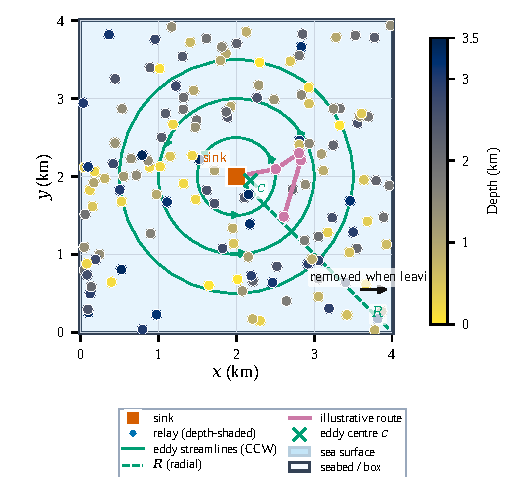
\includegraphics[width=\columnwidth]{fig4_deploy_top}
\caption{Deployment used in the evaluation (one placement, seed 20261801; top view, relays shaded by depth). The sink and the eddy centre coincide. The route and the eddy streamlines are illustrative.}
\label{fig:deploy}
\end{figure}

\emph{Scenarios.} Scenario~I is static. Scenario~II applies the eddy and Gauss--Markov flow of Section~\ref{sec:network} with a peak speed of 0.15~m/s, and Scenario~GM2 doubles the speed and the variability. A relay that leaves the volume is removed, which affects on average 22.3\% of the relays in II and 29.5\% in GM2. We had aimed at 15\% and report the measured fractions.

\emph{Intervals and estimators.} The packet cohort, the energy interval, and the control count are different intervals (Section~\ref{sec:metrics}): packets generated in $[900,14400)$~s, energy in $[900,14700]$~s, and control frames starting in $[0,14400]$~s. The primary estimator is the mean of run-level ratios, not the pooled ratio; a pooled sensitivity analysis for QELAR gives energy differences of $-181$, $-20$, and $-24$~mJ/bit against 120~s periodic in Scenarios I, II, and GM2, with the same sign pattern and bootstrap intervals that exclude zero only in Scenario~I.

\emph{Statistics.} MARV uses evaluation seeds 20261801--40 (40 per cell; the scalability and drift sweeps use the first ten) and QELAR uses 20261841--80. DA-HELLO configurations were locked on separate tuning seeds (20261114--23) that appear in no evaluation table. Comparisons are paired by seed. Non-inferiority is stated against an explicit margin: 0.5 percentage points (pp) for MARV, and 3~pp for QELAR, because the paired standard deviation of PDR differences on QELAR was 6--10~pp in the pilot, against below 1~pp on MARV. The QELAR margin was therefore chosen after the pilot and before the evaluation. Holm correction is applied within each pre-registered family of three scenarios; the intervals shown are unadjusted.

\subsection{Hosts, Arms, and Pre-Registered Statements}
\label{sec:arms}
\emph{Hosts.} MARV and QELAR are our re-implementations of the published rules. They carry state in data headers; for each we also run a labelled HELLO-only variant in which header attributes are stripped from data frames and only HELLO or beacon decodes write records. The variants are not reproductions of a published protocol.

\emph{Arms} (Table~\ref{tab:arms}). Every arm shares the host's routing logic and the same join announcement and 60~s sink beacon; only HELLO scheduling differs. B0 sends nothing after joining. Periodic arms send a jittered HELLO every $T$~s and receive one free full round at time zero, which favours them; $T=120$~s is the comparator in the pre-registered statements. The Trickle arm is tuned on MARV but uses the host's own timer defaults on QELAR, so the two Trickle results are not matched comparisons. The DA-HELLO configuration differs by host class and was locked on the tuning seeds.

\emph{Statements.} S1 (MARV HELLO-only): DA-HELLO is non-inferior to periodic 120~s in PDR at 0.5~pp and uses at least 50\% fewer control bytes. S1$'$: non-inferior in PDR, with fewer control bytes and lower energy per bit. S2 (MARV header): non-inferior to B0 at 0.5~pp with an energy change below 5\%. Q1, Q1$'$ (QELAR HELLO-only): as S1 and S1$'$ at 3~pp and at least 40\% fewer bytes. Q2: B0 is more than 5~pp below DA-HELLO. Q3 (QELAR header): non-inferior to the host alone at 3~pp with an energy change below 5\%.


\subsection{Results: HELLO-Only Hosts}
\label{sec:res-hello}
Fig.~\ref{fig:pareto} plots delivery against control overhead. Without HELLOs, both hosts collapse: B0 delivers 0.14 to 0.18 on MARV and 0.06 to 0.07 on QELAR, because no record is created after joining. Periodic HELLOs restore routing, but frequent ones hurt: on MARV, delivery in Scenario~I rises from 0.45 at 20~s (376~B/s) to 0.78 at 120~s (64~B/s), since HELLO traffic congests the shared channel, and the 5~s and 10~s periods saturate it (0.01 and 0.13 in Scenario~II, at 1275 and 647~B/s).

\begin{figure*}[!t]
\centering
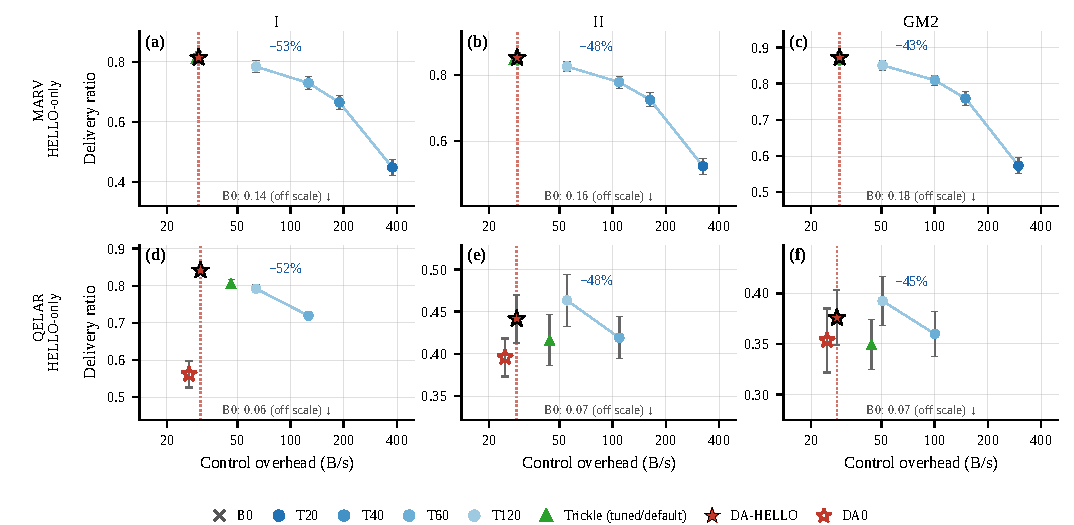
\includegraphics[width=\textwidth]{fig5_pareto}
\caption{Delivery versus control overhead on hosts whose state travels only in HELLOs (top: MARV variant; bottom: QELAR variant); $n=40$ seeds, bars are 95\% intervals. The no-HELLO value is off scale and printed in each panel. $y$-axes differ between panels. Percentages give the control bytes of DA-HELLO relative to periodic 120~s.}
\label{fig:pareto}
\end{figure*}

\begin{table*}[!t]
\caption{Pre-Registered Comparisons (MARV t103 Seeds $20261801$--$40$;
QELAR t109 Phase~2 Seeds $20261841$--$80$). $\Delta$ Is DA-HELLO Minus the
Named Reference; Intervals Are Paired Student-$t$ $95\%$.}
\label{tab:prereg}
\centering
\scriptsize
\setlength{\tabcolsep}{4pt}
\begin{tabular*}{\textwidth}{@{\extracolsep{\fill}}llrrr@{}}
\hline
Stmt & Sc & $\Delta$PDR [pp] & Rel.\ bytes & $\Delta E_{\mathrm{bit}}$ [mJ/bit] \\
\hline
\multicolumn{5}{l}{\emph{S1/S1$'$: MARV HELLO-only vs jittered T120}}\\
S1  & I   & $+3.01$ [$2.51$, $3.51$] & $-52.7\%$ & $-140$ [$-152$, $-128$] \\
    & II  & $+2.64$ [$1.99$, $3.29$] & $-47.6\%$ & $-121$ [$-132$, $-109$] \\
    & GM2 & $+2.15$ [$1.61$, $2.68$] & $-42.8\%$ & $-104$ [$-114$, $-95$] \\
\hline
\multicolumn{5}{l}{\emph{S2: MARV header vs B0}}\\
S2  & I   & $+0.60$ [$0.01$, $1.19$] & --- & rel $-0.1\%$ [$-0.9$, $+0.7$] \\
    & II  & $+0.64$ [$0.09$, $1.18$] & --- & rel $-0.0\%$ [$-0.7$, $+0.6$] \\
    & GM2 & $+0.44$ [$0.14$, $0.74$] & --- & rel $+0.4\%$ [$+0.1$, $+0.7$] \\
\hline
\multicolumn{5}{l}{\emph{Q1/Q1$'$: QELAR HELLO-only DA480 vs T120}}\\
Q1  & I   & $+4.95$ [$4.03$, $5.88$] & $-51.5\%$ & $-182$ [$-201$, $-163$] \\
    & II  & $-2.19$ [$-4.38$, $+0.00$] & $-48.1\%$ & $-30$ [$-145$, $+86$] \\
    & GM2 & $-1.67$ [$-3.65$, $+0.32$] & $-44.9\%$ & $+11$ [$-139$, $+161$] \\
\hline
\multicolumn{5}{l}{\emph{Q2: QELAR HELLO-only DA480 $-$ B0}}\\
Q2  & I   & $+78.2$ [$77.3$, $79.2$] & --- & B0 collapses \\
    & II  & $+37.2$ [$34.5$, $39.9$] & --- & \\
    & GM2 & $+30.5$ [$28.1$, $32.9$] & --- & \\
\hline
\multicolumn{5}{l}{\emph{Q3: QELAR header (FC off, $m{=}10$) vs alone}}\\
Q3  & I   & $+0.16$ [$-0.08$, $+0.40$] & --- & rel $E_{\mathrm{bit}}$ hi $+0.1\%$ \\
    & II  & $-0.41$ [$-2.42$, $+1.60$] & --- & rel $E_{\mathrm{bit}}$ hi $+4.3\%$ \\
    & GM2 & $+0.31$ [$-2.03$, $+2.65$] & --- & rel $E_{\mathrm{bit}}$ hi $+4.6\%$ \\
\hline
\end{tabular*}
\end{table*}


On MARV, DA-HELLO delivers 2.1 to 3.0~pp more than periodic 120~s, with 43 to 53\% fewer control bytes and 8 to 10\% lower energy per bit (Table~\ref{tab:prereg}); all intervals exclude zero. S1$'$ and the B0 contrast are met in every scenario, but S1 as written is met in Scenario~I only, because the byte saving falls to 47.6\% and 42.8\% in II and GM2, below the pre-registered 50\%. Against the tuned Trickle, DA-HELLO is within 0.25 to 0.60~pp of delivery, with a control rate within 4.5\% and 0.9 to 1.8\% lower energy per bit (the delivery interval excludes zero in II and GM2): it ties Trickle and does not beat it.

On QELAR the result is mixed. In Scenario~I, DA-HELLO gains 4.95~pp over periodic 120~s with 51.5\% fewer bytes and 13\% lower energy per bit. In II and GM2 it is 2.2 and 1.7~pp lower, with 48\% and 45\% fewer bytes. The lower bounds ($-4.4$ and $-3.7$~pp) fall below the 3~pp margin, so non-inferiority is not shown, and the energy difference has an interval that spans zero. Periodic 120~s therefore keeps a small delivery edge there at about twice the overhead. Against the other comparators DA-HELLO is clearly better: relative to the host's default Trickle it delivers 3.6, 2.5, and 2.7~pp more (the interval excludes zero in I and GM2) with 33 to 36\% fewer bytes and about 8\% lower energy per bit, and relative to periodic 60~s it uses 72 to 76\% fewer bytes and 14 to 28\% less energy per bit.

Table~\ref{tab:causes} shows where the HELLOs come from. First-contact replies account for most of them (5055 of about 8160 starts per run on MARV and 4679 of 8094 on QELAR in Scenario~II), the slow refresh for most of the rest, and membership and score-change requests together for under 160 per run.


\subsection{Results: Hosts With State in Data Headers}
\label{sec:res-header}
When data frames already carry the state, extra HELLOs add little and cost delivery (Fig.~\ref{fig:header}). On MARV, periodic HELLOs lose 37, 33, and 30~pp at 20~s and 4.3, 2.9, and 2.9~pp at 120~s relative to B0 in Scenarios I, II, and GM2, and the tuned Trickle loses 0.4 to 0.8~pp. DA-HELLO is slightly above B0 (+0.60, +0.64, and +0.44~pp), and its energy per bit differs from B0 by at most 0.42\%, so S2 is met; it also beats the tuned Trickle by 1.0 to 1.3~pp with about half the control bytes. We read this as no harm relative to doing nothing, not as a gain.

QELAR shows the same ordering with larger penalties: periodic 60~s loses 12.5, 13.7, and 14.2~pp, periodic 120~s loses 4.1, 6.3, and 7.1~pp, and the default Trickle loses 1.1, 8.0, and 11.6~pp. DA-HELLO with the first-contact reply on loses 0.2, 10.1, and 15.2~pp, and sends about 2900 first-contact HELLOs per run (Table~\ref{tab:causes}); with the reply off it is indistinguishable from the host alone (+0.16, $-0.41$, and +0.31~pp; Q3 is met) and sends about 12 membership HELLOs per run. We use the second configuration on QELAR's header regime. The two settings also differ in the rank margin, so this is a joint-configuration contrast, and we did not isolate why the reply is harmless on MARV but harmful on QELAR.

\begin{figure*}[!t]
\centering
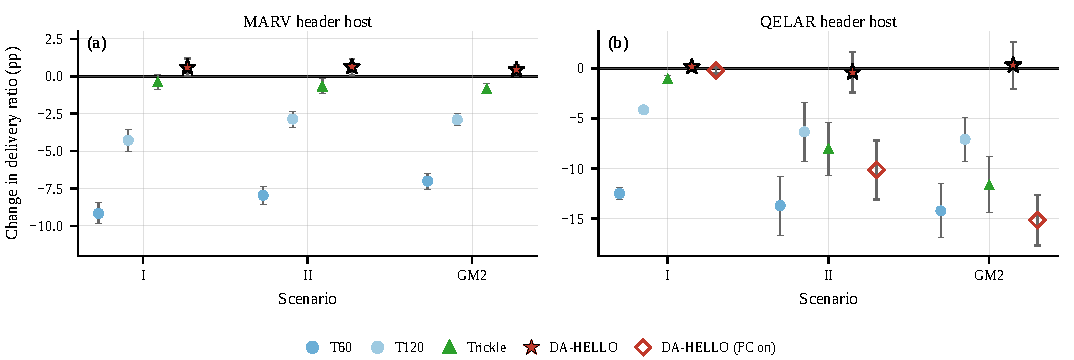
\includegraphics[width=\textwidth]{fig6_header}
\caption{Change in delivery relative to sending no HELLOs after joining (MARV) or to the host alone (QELAR), for hosts that carry state in data headers ($n=40$ per cell, paired 95\% intervals). The 20~s and 40~s MARV arms (losses of 12 to 37~pp) are omitted for scale. With first contact on, DA-HELLO on QELAR loses 10 to 15~pp in II and GM2.}
\label{fig:header}
\end{figure*}

\subsection{Components, Scalability, and Drift}
\label{sec:ablate}
\emph{Slow refresh.} On the MARV HELLO-only host, removing the 480~s refresh lowers delivery by 4.4, 1.8, and 1.3~pp in Scenarios I, II, and GM2 (all intervals exclude zero) and saves 5.6 to 9.1~B/s. A 240~s refresh lowers delivery by 0.8, 0.5, and 0.5~pp relative to 480~s and costs 10 to 14~B/s more (Fig.~\ref{fig:refresh}). On QELAR the same removal costs 28.0, 4.5, and 2.2~pp. The refresh therefore carries most of the delivery beyond first contact on HELLO-only hosts, and it is one reason why the configuration differs between regimes.

\emph{Score-change test.} The test raised between 12 and 160 host-state requests per run (Table~\ref{tab:causes}); on QELAR HELLO-only about 144 per run, roughly one per node, whereas the header configuration with the test off raised none. These are request counters, not transmissions, and we have no matched rank-on and rank-off comparison, so no performance benefit is attributed to the test or to the back-off.

\begin{figure}[!t]
\centering
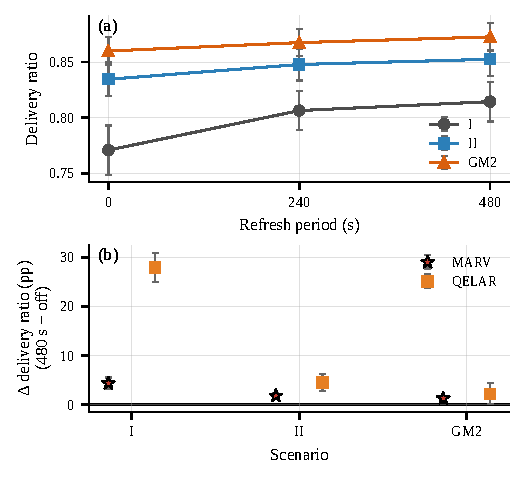
\includegraphics[width=\columnwidth]{fig7_refresh}
\caption{Slow-refresh ablation. (a) MARV HELLO-only delivery for refresh periods of 0, 240, and 480~s. (b) Paired gain of the 480~s refresh over no refresh, for MARV and QELAR ($n=40$, 95\% intervals).}
\label{fig:refresh}
\end{figure}

\begin{figure}[!t]
\centering
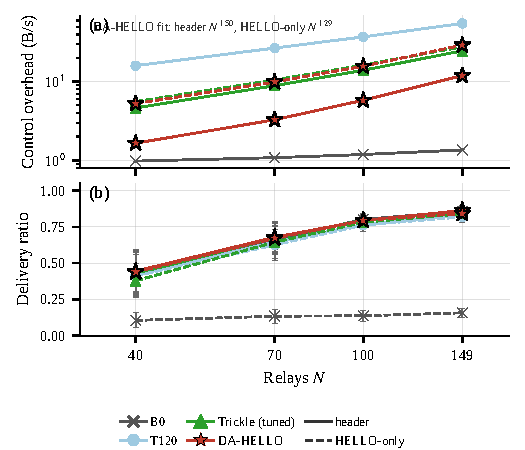
\includegraphics[width=\columnwidth]{fig8_scale}
\caption{Scalability in Scenario~II ($n=10$ seeds per point). Control overhead grows roughly as $N^{1.5}$ for DA-HELLO on the header host and $N^{1.3}$ on the HELLO-only host, below periodic 120~s and the tuned Trickle; delivery is low at 40 and 70 relays for all policies.}
\label{fig:scale}
\end{figure}

\emph{Scalability.} Fig.~\ref{fig:scale} varies the number of relays from 40 to 149 in Scenario~II (ten seeds per point). The overhead of DA-HELLO grows from 1.7 to 12.4~B/s on the header host and from 5.1 to 29.3~B/s on the HELLO-only host, which corresponds to power laws with exponents of about 1.5 and 1.3 in $N$. Periodic 120~s grows from 15 to 53~B/s and the tuned Trickle from 4.8 to 26.6~B/s (header host). Delivery is low for every policy at 40 and 70 relays (0.42 to 0.44 and 0.66 to 0.69 on the header host), owing to sparse connectivity and relay removal, and DA-HELLO stays within 0.1~pp of the best comparator at 100 relays. The energy per bit at 40 relays is not reported because one zero-delivery run has no defined value.


\emph{Drift speed.} Across mean speeds of 0.10, 0.15, 0.30, and 0.50~m/s (ten seeds), DA-HELLO delivers 0.839, 0.843, 0.859, and 0.867 on the HELLO-only host, against 0.813, 0.819, 0.835, and 0.843 for periodic 120~s and 0.832, 0.841, 0.852, and 0.861 for the tuned Trickle. On the header host it delivers 0.858, 0.863, 0.874, and 0.888, against 0.854, 0.858, 0.872, and 0.877 for B0.


\begin{table*}[!t]
\caption{DA-HELLO HELLO Starts by Cause in Scenario~II ($n=40$ Seed Means).
First-Contact Replies Dominate; Slow Refresh Accounts for Most of the
Remainder on HELLO-Only Hosts. Membership and Score-Change Requests
Together Stay Under 160 per Run.}
\label{tab:causes}
\centering
\scriptsize
\setlength{\tabcolsep}{5pt}
\begin{tabular*}{\textwidth}{@{\extracolsep{\fill}}lrrrrp{0.28\textwidth}@{}}
\hline
Host / arm & HELLO tx & FC reply & Refresh & Mem./rank & Notes \\
\hline
MARV HELLO-only & 8160 & 5055 & 2836$^{\mathrm{a}}$ & 44 & refresh$=$480\,s \\
QELAR HELLO-only & 8094 & 4679 & 3742 & 158 & mem 14, rank 144 \\
QELAR header (FC off) & --- & 0 & 0 & 14 & $\approx$12 membership \\
QELAR header (FC on) & --- & 2907 & 0 & 141 & descriptive \\
MARV header & 3155 & 2981 & 0$^{\mathrm{a}}$ & 24 & refresh$=$0 \\
\hline
\multicolumn{6}{l}{\footnotesize $^{\mathrm{a}}$MARV export codes slow-refresh and residual adaptive starts in \texttt{cause\_other}.}\\
\end{tabular*}
\end{table*}


\subsection{Pilot Runs on Further Hosts}
\label{sec:pilots}
Before the campaign, a host had to deliver at least 0.30 of its packets in Scenario~II without any HELLO scheduler on five tuning seeds. QELAR qualified (0.665 after aligning its candidate gate and previous-hop rule with its paper, up from 0.385). SAQR delivered 0.082 and LQARP 0.284 with an interval that spans the threshold, so neither was campaigned and we make no claim about DA-HELLO on them.

\subsection{Limitations and Disclosures}
\label{sec:limits}
The evidence supports a bounded statement. Where state travels only in HELLOs, DA-HELLO saves 43 to 53\% of the control bytes of periodic 120~s and delivers more on MARV; on QELAR it is competitive but not shown non-inferior in the drifting scenarios. Where state travels in headers, it matches doing nothing, and on QELAR only with first contact off. The configuration therefore differs by host class and is not self-adapting.

Several choices limit these results. Both hosts are our re-implementations, and 35 of 65 checklist rows of the host audit match the papers; the HELLO-only variants are constructed. Periodic arms receive a free first round, and B0 includes the sink beacon. Header bits that hosts add to data frames are not charged. The relay-removal fractions (22\% and 30\%) exceed the 15\% target and the removal rule affects the mobile scenarios. On QELAR, the pilot suggested +2.3 and +0.5~pp against periodic 120~s, but the evaluation gave $-2.2$ and $-1.7$~pp, and the 3~pp margin was set after the pilot. A matched first-contact and rank ablation, equalised start-up for the periodic arms, and a field-aware controller remain future work. The MARV raw run logs are no longer available, so MARV results rest on the retained exports. First-contact replies have a precedent in APU~\cite{chen2013apu}, and the void-triggered beacon in earlier void-handling work~\cite{ghoreyshi2017void}.
